\section{Topologia di interconnessione}
Poniamoci ora nel caso di architetture multicomputer, in cui a differenza di quelle multiprocessore, non esiste memoria condivisa né un bus comune, ma la comunicazione tra i processori dipende dalla \textbf{topologia di rete}, in particolare dal diametro (massima distanza tra due nodi).
Questo rende più complesso ridurre i costi di comunicazione, poiché spesso non è possibile ottenere una totale connettività. Un'ulteriore difficoltà riguarda l'allocazione dei processi: quando i processi sono più dei processori, è necessario bilanciare la comunicazione e l’uso delle risorse.
Idealmente, si dovrebbero:
\begin{itemize}
    \item Assegnare allo stesso nodo i processi che comunicano spesso.
    \item Distribuire su nodi diversi quelli che richiedono molte risorse computazionali.
\end{itemize}
Per ottimizzare l'allocazione servono funzioni obiettivo specifiche, ma la loro definizione è complessa perché dipende dai dati trattati dai processi.
\\
\\
Nell'ottica in cui ci poniamo (punto di vista puramente hardware), la configurazione descritta 
dall'architettura non può risolvere il problema dall'allocazione dei processi, ma può far fronte a 
quello della connettività, cercando di rendere quanto più semplice possibile la comparazione tra 
grafo del problema e quello dell'architettura.  
Esistono due soluzioni, le \textit{reti dirette} e \textit{reti indirette}.
\\
\\
Le \textbf{reti dirette} definiscono una topologia fissa, per cui la compatibilità tra i grafi è realizzata in maniera analitica attraverso l'utilizzo di formule provenienti dal campo della ricerca operativa. Le \textbf{reti indirette}, invece, sono realizzate attraverso particolari dispositivi chiamati 
\textit{switch}, che consentono di ottenere una totale connettività attraverso un 
sistema dinamico di comunicazione. Per capire meglio come questo sia possibile, è necessario approfondire alcuni dettagli di realizzazione sugli switch. Innanzitutto, l'obbiettivo principale di questi dispositivi è gestire dei conflitti, ovvero di situazioni in cui due o più nodi cercano di comunicare contemporaneamente con un altro. A questo proposito, è possibile classificare gli switch in due categorie:
\begin{itemize}
    \item A \textbf{singolo stadio} (Diretti).
    \item A \textbf{N stadi} (Indiretti).
\end{itemize}
Per creare uno \textbf{switch a connessione diretta} tra due nodi diversi, è necessario avere due informazioni: l'indirizzo del nodo sorgente e quello del nodo destinazione. Il dispositivo che si vuole realizzare dovrà avere \(N\) nodi in ingresso ed \(N\) nodi in uscita. Per poter implementare tale architettura si deve scomporre il sistema in due sottosistemi diversi, quello di ingresso e quello di uscita. Tale suddivisione viene realizzata mediante multiplexer e demulitplexer, entrambi generalmente realizzati in logica three-state [\ref{fig:switch-dir}]. 
\begin{figure}[!h]
    \centering
    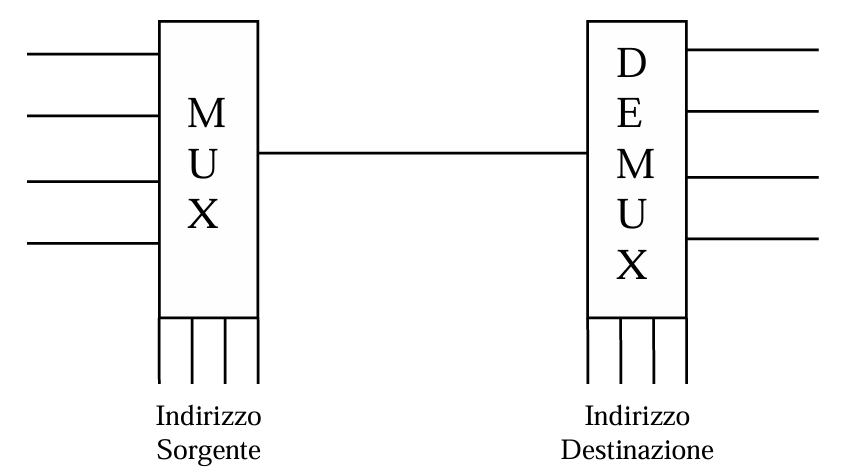
\includegraphics[width=0.35\linewidth]{img/switch_dir.png}
    \caption{Switch a singolo stadio.}
    \label{fig:switch-dir}
\end{figure}
L'inconveniente implicito del meccanismo implementato, è che automaticamente si realizza una mutua esclusione tra i nodi dovuta al fatto che, potrà essere attivo un solo collegamento per volta. Quindi, per realizzare un collegamento di \(N/2\) comunicazioni simultanee, si dovrà replicare l'hardware \(N/2\) volte. Le caratteristiche che rendono favorevole questa soluzione sono: assenza di stadi intermedi, buona efficienza, basso parallelismo e parallelismo fisico ottenuto riproducendo lo stesso elemento più volte.
\\
\\
La soluzione trovata non è esente dal problema dei conflitti, poiché aumentando il parallelismo in 
hardware si va semplicemente a rendere possibile la comunicazione parallela, ma se i nodi di 
ingresso vogliono comunicare con lo stesso nodo di uscita è inevitabile che si creano collisioni. 
Si rende necessario, quindi, predisporre un gestore dei conflitti. La soluzione con \textbf{switch indiretti}, si basa su una serie di stadi intermedi per stabilire la comunicazione tra più nodi. Sono state proposte nel tempo varie topologie per implementare tale logica, ad esempio è facile rendersi conto che, utilizzando dispositivi a due ingressi e due uscite per realizzare gli stadi, con 
\(Log_2n\) stadi è possibile risolvere il problema della connettività, avendo tra l'altro il vantaggio di usare blocchi molto semplici che devono solo decidere se 
procedere in una direzione o in un'altra. Ovviamente esiste un problema non banale, come si fa a collegare i blocchi tra di loro (indirizzamento)?. Per switch a connessione diretta l’indirizzamento è semplice perché gli indirizzi vanno direttamente nel multiplexer e nel demultiplexer per creare il path. Nel caso di architetture multistadio invece, l'indirizzo disposto in \(k\) bit, deve essere diviso in tante parti quanti sono gli stadi, in modo da comandare opportunamente i blocchi. Questo significa che non esiste una logica di controllo centralizzata come nel caso precedente, ma la logica di controllo è distribuita negli stadi. Ovviamente è una condizione abbastanza forte dal punto di vista dell'architettura, che è possibile realizzare soltanto utilizzando particolari proprietà topologiche della rete. Un esempio che implementa una soluzione molto interessante è rappresentata dalla \textbf{Omega Newtork}, la quale si basa sul concetto del \textit{perfect shuffling} [\ref{fig:omega}].  
\begin{figure}[!h]
    \centering
    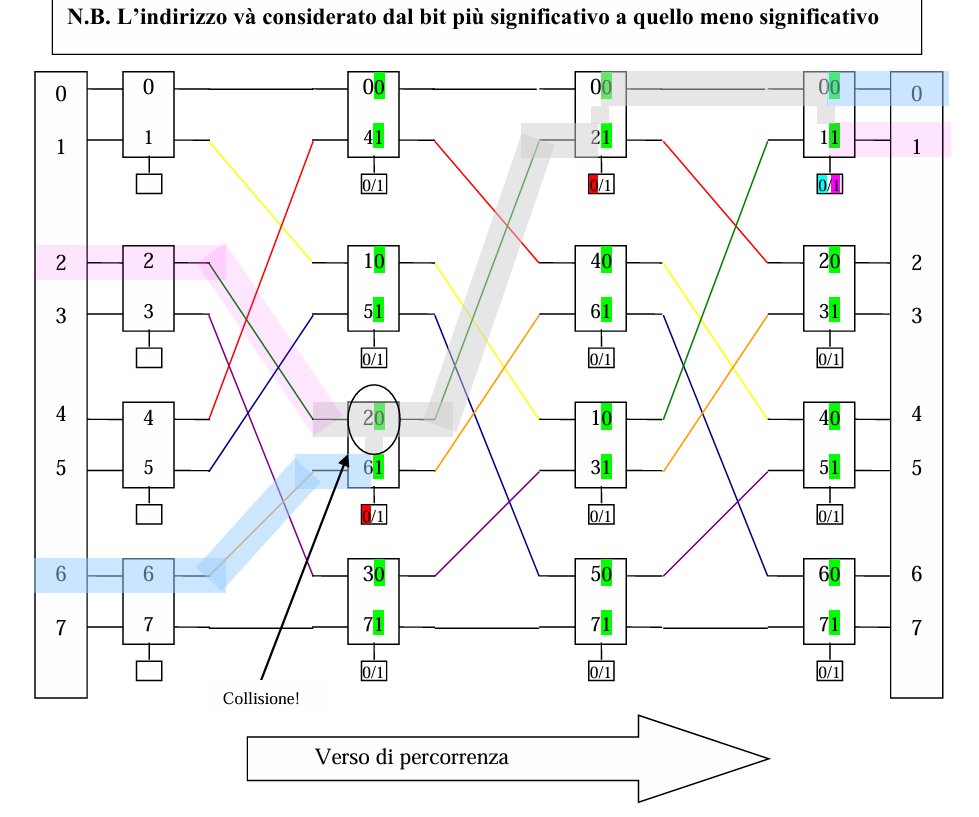
\includegraphics[width=0.6\linewidth]{img/omeganet.png}
    \caption{Switch a \(N\) stadi con omega network.}
    \label{fig:omega}
\end{figure}
Il vantaggio evidente, come detto prima, risiede nella semplicità dei componenti usati per realizzare il dispositivo che implementa il routing, ovvero blocchi con due ingressi e due uscite. L’unica nota negativa, invece, risulta proprio l'utilizzo di più stadi. Va notato che, la flessibilità indotta dall'architettura, grazie alla forte modularità dei componenti, rende lo switch molto scalabile, infatti  è facile realizzarne uno di grandi dimensioni, cosa che non è semplicemente possibile per gli switch diretti. Il problema che si verifica è, però sempre lo stesso, se due nodi di ingresso vogliono parlare con lo stesso nodo di uscita simultaneamente generano un conflitto, inoltre la contesa può anche avvenire nei nodi intermedi. Per comprendere come gestire tali conflitti, ricordiamo che la comunicazione può avvenire secondo due modalità:
\begin{itemize}
    \item \textbf{Wormhole}: Il pacchetto viene suddiviso in piccole unità, appena la prima (di solito l’header) arriva a uno switch, può essere subito inoltrata anche se il resto del pacchetto non è ancora arrivato. Lo svantaggio è che può provocare deadlock se molti pacchetti competono per le stesse risorse. I vantaggi sono una latenza più bassa (opo che l'header ha conquistato il canale i successivi frammenti viaggiano senza ritardi) e buffer di dimensioni minori. Cosa accade se il flusso di frammenti si blocca, ad esempio a causa di un conflitto? Esistono quattro soluzioni:
    \begin{enumerate}
        \item \textbf{Blocco conservativo}: Il messaggio si ferma finché il problema non si risolve. È semplice ma può bloccare molti nodi. 
        \item \textbf{Distruzione del messaggio}: Il messaggio viene eliminato. Rete con possibile perdita di dati.
        \item \textbf{Re-instradamento}: Si cerca un percorso alternativo, ma è possibile solo in reti non statiche e con topologie flessibili (quindi non per omega network). Inoltre, in questo caso i pacchetti possono arrivare fuori ordine, quindi serve una strategia software che si occupi di riordinarli. 
        \item \textbf{Cut-through}: Il nodo blocca memorizza temporaneamente i dati, mischiando wormhole e store and forward. Serve però un minimo di buffer (es. shift-register e contatore).
    \end{enumerate}
    \item \textbf{Store \& Forward}: Ogni nodo intermedio deve riceve interamente il pacchetto, e solo dopo lo memorizza (store) e lo inoltra (forward) al nodo successivo. Gli svantaggi sono i tempi di ritardo e la necessità di buffer per memorizzare le informazioni.
\end{itemize}
La differenza chiave tra i due è quindi che nel wormhole c'è una negoziazione del percorso, il quale è dinamico e dipende dal primo frammento, mentre nello store and forward  la negoziazione di tratta, ovvero avviene a ogni stadio.
